\documentclass[12pt]{article}
\usepackage[top=1in, bottom=1in, left=1in, right=1in]{geometry}

\usepackage{setspace}
\onehalfspacing

\usepackage{amssymb}
%% The amsthm package provides extended theorem environments
\usepackage{amsthm}
\usepackage{epsfig}
\usepackage{times}
\renewcommand{\ttdefault}{cmtt}
\usepackage{amsmath}
\usepackage{graphicx} % for graphics files
\usepackage{tabu}

% Draw figures yourself
\usepackage{tikz} 

% writing elements
\usepackage{mhchem}

\usepackage{paralist}

% The float package HAS to load before hyperref
\usepackage{float} % for psuedocode formatting
\usepackage{xspace}

% from Denovo Methods Manual
\usepackage{mathrsfs}
\usepackage[mathcal]{euscript}
\usepackage{color}
\usepackage{array}

\usepackage[pdftex]{hyperref}
\usepackage[parfill]{parskip}

% math syntax
\newcommand{\nth}{n\ensuremath{^{\text{th}}} }
\newcommand{\ve}[1]{\ensuremath{\mathbf{#1}}}
\newcommand{\Macro}{\ensuremath{\Sigma}}
\newcommand{\rvec}{\ensuremath{\vec{r}}}
\newcommand{\vecr}{\ensuremath{\vec{r}}}
\newcommand{\omvec}{\ensuremath{\hat{\Omega}}}
\newcommand{\vOmega}{\ensuremath{\hat{\Omega}}}
\newcommand{\even}{\ensuremath{\phi^g}}
\newcommand{\odd}{\ensuremath{\vartheta^g}}
\newcommand{\evenp}{\ensuremath{\phi^{g'}}}
\newcommand{\oddp}{\ensuremath{\vartheta^{g'}}}
\newcommand{\Sn}{\ensuremath{S_N} }
\newcommand{\Ye}[2]{\ensuremath{Y^e_{#1}(\vOmega_#2)}}
\newcommand{\sigg}[1]{\ensuremath{\Macro^{gg'}_{s\,#1}}}
\newcommand{\psig}{\ensuremath{\psi^g}}
%---------------------------------------------------------------------------
%---------------------------------------------------------------------------
\begin{document}
\begin{center}
{\bf NE 255, Fa16 \\
Equation Discretization\\
September 22 and 27, 2016}
\end{center}

\setlength{\unitlength}{1in}
\begin{picture}(6,.1) 
\put(0,0) {\line(1,0){6.25}}         
\end{picture}

Start from the general time-dependent NTE without delayed neutrons, with 7 independent variables. We need to discretize each variable.	
%
\begin{align}
&\frac{1}{v}\frac{\partial \psi}{\partial t}(\rvec,E,\omvec,t) + 
\omvec\cdot  \nabla \psi(\rvec,E,\omvec,t)+
\Sigma_t(\rvec,E)\psi(\rvec,E,\omvec,t)
\\& \quad\quad\quad\quad =
\int_0^{\infty}\int_{4\pi}\Sigma_s(\rvec, E'\rightarrow E,\omvec'\rightarrow\omvec)
\psi(\rvec,E',\omvec',t)d\omvec'dE'\nonumber
\\&\quad\quad\quad\quad\quad\quad +\frac{\chi_p(E)}{4\pi}\int_0^{\infty}\int_{4\pi}\nu(E')\Sigma_f(\rvec,E')
\psi(\rvec,E',\omvec',t)d\omvec'dE'\nonumber
\\&\quad\quad\quad\quad\quad\quad\quad\quad+S(\rvec, E, \omvec,t)\nonumber.
\end{align}

\subsection*{Time}
Discretize the time interval $[0, T]$ into $N$ timesteps:
%
\begin{figure}[h!]
    \begin{center}
    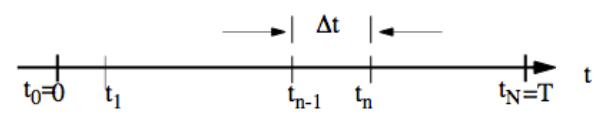
\includegraphics[keepaspectratio, width = 3.5 in]{time}
    \end{center}
\end{figure}
%
Integrate the equation from $t=t_{n-1}$ to $t = t_n$, where we will use the following definitions:
\begin{align*}
\psi(\vec{r}, E ,\vOmega, t_n) &= \psi_n(\vec{r}, E ,\vOmega)\\
\Delta t &= t_{n} - t_{n-1}\\
\bar{\psi}(\vec{r}, E ,\vOmega) &= \frac{1}{\Delta t} \int_{t_{n-1}}^{t_n} dt\: \psi(\vec{r}, E ,\vOmega, t)
\end{align*}
(Note: we're not specifying what actually happens in the integration; we're generically defining a time-averaged angular flux).

We also need to handle the time derivative term so that we can approximate it on a time grid. We will use \textit{First Order Backward Difference} (more on that later): 
\[
\frac{1}{v} \frac{\partial \psi}{\partial t}(\rvec,E,\omvec,t) = \frac{1}{v}\frac{\psi_n(\vec{r}, E ,\vOmega) - \psi_{n-1}(\vec{r}, E ,\vOmega)}{\Delta t}
\]
To get the time behavior of the solution, we integrate the entire transport equation over each time step
\[
\int_{t_{n-1}}^{t_n} dt\: [\cdot]
\]
noting
\[
\int_{t_{n-1}}^{t_n} dt\: \bigl(\frac{1}{v}\frac{\psi_n(\vec{r}, E ,\vOmega) - \psi_{n-1}(\vec{r}, E ,\vOmega)}{\Delta t}\bigr) = \frac{1}{v}\frac{\psi_n(\vec{r}, E ,\vOmega) - \psi_{n-1}(\vec{r}, E ,\vOmega)}{\Delta t}
\]
which gives
\begin{align*}
\frac{1}{v}&\frac{\psi_n(\vec{r}, E ,\vOmega) - \psi_{n-1}(\vec{r}, E ,\vOmega)}{\Delta t} 
+ \omvec\cdot  \nabla  \bar{\psi}(\vec{r}, E ,\vOmega) 
+ \Sigma_t(\rvec,E)\bar{\psi}(\vec{r}, E ,\vOmega) 
= \\& \int_0^{\infty}dE'\int_{4\pi}d\omvec'\: \Sigma_s(\rvec, E'\rightarrow E,\omvec'\rightarrow\omvec) \bar{\psi}(\vec{r}, E' ,\vOmega')
\\&+ \frac{\chi_p(E)}{4\pi}\int_0^{\infty}dE'\:\nu(E')\Sigma_f(\rvec,E')\int_{4\pi}d\omvec'\:
\bar{\psi}(\vec{r}, E' ,\vOmega')
+\bar{S}(\rvec, E, \omvec)
\end{align*}
Note(!): we now have two unknowns ($\psi_n$ and $\bar{\psi}$). We need to relate them; we choose a linear combination with a weighting parameter, $\beta$:
\[
\bar{\psi} = \beta \psi_n + (1 - \beta)\psi_{n-1}
\]
We substitute this in to get
\begin{align*}
\omvec\cdot  \nabla  \bar{\psi}(\vec{r}, E ,\vOmega) 
&+ \bigl(\Sigma_t + \frac{1}{v \beta \Delta t}\bigr)\bar{\psi}(\vec{r}, E ,\vOmega) 
=  \frac{1}{v \beta \Delta t} \psi_{n-1}(\vec{r}, E ,\vOmega) \\
&+ \int_0^{\infty}dE'\int_{4\pi}d\omvec'\: \Sigma_s(\rvec, E'\rightarrow E,\omvec'\rightarrow\omvec) \bar{\psi}(\vec{r}, E' ,\vOmega')
\\&+ \frac{\chi_p(E)}{4\pi}\int_0^{\infty}dE'\:\nu(E')\Sigma_f(\rvec,E')\int_{4\pi}d\omvec'\:
\bar{\psi}(\vec{r}, E' ,\vOmega')
+\bar{S}(\rvec, E, \omvec)
\end{align*}
We solve this for $n=1, \dots, N$ and $\psi_0$ is given (initial value problem!).

%---------------------------------------------------------------------------
\subsubsection*{Aside about Finite Difference}
Finite difference is a common way to numerically approximate derivatives.  \textbf{Example} Given $f$ is $ C^2 \in [a,b]$ and $x_0 \in [a,b]$, find an approximation to $f'(x_0)$ and or $f''(x_0)$, etc.

We're going to come at this from \textbf{Taylor's theorem}, which gives an approximation of a k-times differentiable function around a given point by a k-th order Taylor polynomial.
\[
f(x) = \sum_{0}^{k} \frac{f^{(n)}(x_0)}{n!}(x - x_0)^n
\]
% https://en.wikipedia.org/wiki/Taylor%27s_theorem
To approximate any type of derivative to a specified order of accuracy, we Taylor expand several points in our collection. Then, we choose how many points to combine and in what ways. 
\begin{align*}
f(x_0) &= f(x_0)\\
%
f(x_0 \pm h) &= f(x_0) \pm hf'(x_0) + h^2\frac{f''(x_0)}{2} \pm h^3\frac{f'''(x_0)}{6} + f^{(4)}(c_1)\frac{h^4}{24} \\
%
f(x_0 \pm 2h) &= f(x_0) \pm 2h f'(x_0) + 2 h^2 f''(x_0) \pm \frac{4}{3} h^3 f'''(x_0) + \frac{2}{3}h^4 f^{(4)}(c_2)
\end{align*}
We combine the expanded expressions, rearrange to group terms, and solve for what we want:

For \underline{$O(h)$ Backwards Difference}: combine the point and the next point backward:
\begin{align*}
f(x_0) &= f(x_0)\\
f(x_0 - h) &= f(x_0) - hf'(x_0) + h^2\frac{f''(c)}{2}\\
a f(x_0) &+ b f(x_0 - h) = f'(x_0) \\
a f(x_0) &+ b \bigl(f(x_0) - hf'(x_0) + h^2\frac{f''(c)}{2} \bigr) = f'(x_0) \\
(a+b)f(x_0) &-bh f'(x_0) + b h^2\frac{f''(c)}{2} = f'(x_0)
\end{align*}
%
Now, we solve for the coefficients to get what we want
\begin{align*}
a+b = 0 &\quad -bh = 1 \\
b &= -\frac{1}{h} \quad a = \frac{1}{h}
\end{align*}
%
We now sub in $a$ and $b$. This gives the first order ($O(h)$) Backwards Difference approximation, which is what we used for the time derivative.
\begin{align*}
\text{error }&= -\frac{1}{h}h^2\frac{f''(c)}{2}\\
f'(x_0) &= \frac{f(x_0) - f(x_0 - h)}{h} + \frac{1}{2}hf''(\mu)
\end{align*}

A note about what points to choose: you want to think about how your equations transmit information. 
A perturbation of the initial (or boundary) data of an \textit{elliptic or parabolic} equation is felt at once by essentially all points in the domain.
The solutions of hyperbolic equations are ``wave-like." If a disturbance is made in the initial data of a hyperbolic differential equation, then not every point of space feels the disturbance at once.

%---------------------------------------------------------------------------
%---------------------------------------------------------------------------
\subsection*{Energy Discretization}
We'd also like to handle the energy dimension by breaking continuous energy into groups:
\begin{center}
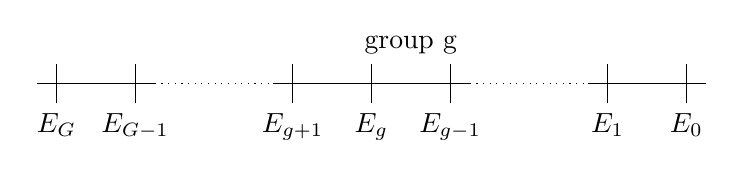
\begin{tikzpicture}
\draw (-.25,0)--(1.25,0);
\draw[dotted] (1.25,0)--(2.75,0);
\draw (2.75,0)--(5.25,0);
\draw[dotted] (5.25,0)--(6.75,0);
\draw (6.75,0)--(8.25,0);
%\draw (4,0)--(5.25,0);
\draw (0,-.25)--(0,.25);
\draw (1,-.25)--(1,.25);
%\draw (2,-.25)--(2,.25);
\draw (3,-.25)--(3,.25);
\draw (4,-.25)--(4,.25);
\draw (5,-.25)--(5,.25);
\draw (7,-.25)--(7,.25);
\draw (8,-.25)--(8,.25);
\node[below] at (0,-.25) {$E_G$};
\node[below] at (1,-.25) {$E_{G-1}$};
\node[below] at (3,-.25) {$E_{g+1}$};
\node[below] at (4,-.25) {$E_g$};
\node[above] at (4.5, .25) {group g};
\node[below] at (5,-.25) {$E_{g-1}$};
\node[below] at (7,-.25) {$E_{1}$};
\node[below] at (8,-.25) {$E_0$};
\end{tikzpicture}
\end{center}
%
We will use the following definitions:
\begin{align*}
\psi_g(\rvec, \vOmega) &\equiv \int_{E_g}^{E_{g-1}} dE\: \psi(\rvec, \vOmega, E) \qquad
\phi_g(\rvec) \equiv \int_{E_g}^{E_{g-1}} dE\: \phi(\rvec,  E)\\
S_g(\rvec, \vOmega) &\equiv \int_{E_g}^{E_{g-1}} dE\: S(\rvec, \vOmega, E) \qquad
\chi_g \equiv \int_{E_g}^{E_{g-1}} dE\: \chi(E)
\end{align*}
%
To perform these integrals, we need to introduce approximations. We \textit{assume the each item is separable in energy}. For example:
\[
\psi(\vec{r}, \vOmega, E) \approx f(E)\psi_g(\vec{r}, \vOmega)\:, \quad E_g < E \leq E_{g-1}\:,
\]
where $f(E)$ is normalized such that $\int_g dE\: f(E) = 1$.

Before we can integrate the whole transport equation over energy, we will need a way to create multigroup cross sections. Options for how to do that in more detail are covered in NE250, so we will do the most common/generic here: weight with the angular flux,
\begin{align*}
\Sigma_{tg}(\vec{r}) &\equiv \frac{\int_{E_g}^{E_{g-1}} dE\: \Sigma_t(\rvec, E) f(E)}{\int_{E_g}^{E_{g-1}} dE\: f(E)} = \frac{\int_{E_g}^{E_{g-1}} dE\: \Sigma_t(\rvec, E) \psi(\rvec, \vOmega, E)}{\int_{E_g}^{E_{g-1}} dE\: \psi(\rvec, \vOmega, E)} \\
&\text{similarly for fission}\\
\Sigma_{s,gg'}(\vOmega' \cdot \vOmega) & \equiv \frac{\int_{E_g}^{E_{g-1}} dE \int_{E_g'}^{E_{g'-1}} dE' \: \Sigma_s(E'\rightarrow E, \vOmega' \cdot \vOmega) f(E')}{\int_{E_g'}^{E_{g'-1}} dE' \: f(E')}\\
& \equiv \frac{\int_{E_g}^{E_{g-1}} dE \int_{E_g'}^{E_{g'-1}} dE' \: \Sigma_s(E'\rightarrow E, \vOmega' \cdot \vOmega) \psi(\rvec, \vOmega', E')}{\int_{E_g'}^{E_{g'-1}} dE' \: \psi(\rvec, \vOmega', E')}
\end{align*}
%
If we use all of those definitions and integrate the TE over energy, we get $g = 0,\dots, G$:
\begin{align*}
[\vOmega \cdot \nabla + \Sigma_{tg}(\vec{r})]\psi_g(\vec{r}, \vOmega) =&  
\sum_{g'=1}^G \int_{4 \pi} d\vOmega'\: \Sigma_{s,gg'}(\vec{r}, \vOmega' \cdot \vOmega) \psi_{g'}(\vec{r}, \vOmega')\\
&+\frac{\chi_g}{4 \pi}\sum_{g'=1}^G \nu\Sigma_{fg'}(\vec{r}) \phi_{g'}(\vec{r}) + q_g(\vec{r}, \vOmega)
\end{align*}
Giving $G+1$ coupled equations. 

These equations are \textbf{exact} in the magical case where (1) the separability in energy holds and (2) the cross sections are constant within each energy group. 


%---------------------------------------------------------------------------
%---------------------------------------------------------------------------
\subsection*{Angular Discretization}
And the complicated one: angle. We have two main approaches, \textbf{Discrete Ordinates} ($S_N$) and \textbf{Spherical Harmonics} (which we often simplify to Legendre polynomials and thus call $P_N$, not to be confused with the scattering expansion).

\subsubsection*{Discrete Ordinates}
The idea of discrete ordinates approximation is that the we change $\omvec$ from continuous to discrete ($\omvec \rightarrow \omvec_n; n = 1,\dots,N)$. Now the TE is only valid along a selected set of angles $\vOmega_n$, and we apply a compatible quadrature (integration approximation) to the integral term. 

Before we get too far into that, we're going to look at \textit{Spherical Harmonics} and how they relate to Legendre polynomials. This will allow us to do angular expansions in three dimensions (derived from the Exnihilo manual and Wikipedia). 

The addition theorem of Spherical Harmonics can be used to evaluate the
Legendre function, $P_l(\vOmega'\cdot\vOmega)$,
\begin{equation}
  P_l(\vOmega'\cdot\vOmega) = \frac{4\pi}{2l+1}\sum_{m=-l}^l
  Y_{lm}(\vOmega)Y^{\ast}_{lm}(\vOmega')\:,
\end{equation}
where the $Y_{lm}$ are
\begin{equation}
  Y_{lm}(\theta,\varphi) = (-1)^m\sqrt
  {
    \frac{2l+1}{4\pi}\frac{(l-m)!}{(l+m)!}
  }\,
  P_{lm}(\cos\theta)\mathrm{e}^{im\varphi}\:,
  \label{eq:complete-spherical-harmonics}
\end{equation}
where the $P_{lm}$ are the \textit{associated Legendre Polynomials}.These are the solutions to
\[
(1-x^{2}){\frac {d^{2}}{dx^{2}}}P_{\ell }^{m}(x)-2x{\frac {d}{dx}}P_{\ell }^{m}(x)+\left[\ell (\ell +1)-{\frac {m^{2}}{1-x^{2}}}\right]P_{\ell }^{m}(x)=0\:,\]
where the indices $l$ and $m$ are referred to as the degree and order of the associated Legendre polynomial, respectively. [before we had called $l$ $n$ and negleced $m$. This equation has nonzero solutions that are nonsingular on $[-1, 1]$ only if $l$ and $m$ are integers with $0 \leq m \leq l$. When in addition $m$ is even, the function is a polynomial. When $m$ is zero, these functions are identical to the Legendre polynomials. They are not polynomials when $m$ is odd, despite the name. 
%https://en.wikipedia.org/wiki/Associated_Legendre_polynomials

Everything in our equations must be real; therefore, we can follow a methodology that shows expands a real-valued function using complex Spherical Harmonics.  First,
the expansion is split into positive and negative components of $m$,
\begin{equation}
  P_l(\vOmega'\cdot\vOmega) = \frac{4\pi}{2l+1}
  \Bigl[
  Y_{l0}(\vOmega)Y_{l0}(\vOmega') +
  \sum_{m=1}^l
  \bigl(Y_{lm}(\vOmega)Y^{\ast}_{lm}(\vOmega') +
  Y_{l-m}(\vOmega)Y^{\ast}_{l-m}(\vOmega')\bigr)\Bigr]\:.
\end{equation}

Examining the $m=0$ term gives the following result
\begin{equation}
  Y_{l0} = \sqrt{\frac{2l+1}{4\pi}}\,P_{l0} = Y^e_{l0}\:,
\end{equation}
where
\begin{align}
  Y^e_{lm} &= D_{lm}P_{lm}\cos (m\varphi)\:,\label{eq:Ye}\\
  Y^o_{lm} &= D_{lm}P_{lm}\sin (m\varphi)\:,\label{eq:Yo}\\
  D_{lm} &= (-1)^m\sqrt{(2-\delta_{m0})\frac{2l+1}{4\pi}
    \frac{(l-m)!}{(l+m)!}}\:.
\end{align}

Expanding the Spherical Harmonics into real and imaginary components, the sum over $m>0$ becomes
\begin{equation}
  \sum_{m=1}^l\Bigl(
  \hat{Y}^e_{lm}(\vOmega)\hat{Y}^e_{lm}(\vOmega') +
  \hat{Y}^o_{lm}(\vOmega)\hat{Y}^o_{lm}(\vOmega') +
  \hat{Y}^e_{l-m}(\vOmega)\hat{Y}^e_{l-m}(\vOmega') +
  \hat{Y}^o_{l-m}(\vOmega)\hat{Y}^o_{l-m}(\vOmega')\Bigr)\:,
\end{equation}
where the imaginary terms have been set to zero because our values must be
real. Using (derivation skipped for brevity)
\begin{align}
 \hat{Y}^e_{l-m} &= (-1)^{-m}\hat{Y}^e_{lm} \equiv (-1)^m\hat{Y}^e_{lm} \:\text{ and}\\
 \hat{Y}^o_{l-m} &= -(-1)^m\hat{Y}^o_{lm}\:,
\end{align}
the summation becomes
\begin{equation}
  \sum_{m=1}^l\Bigl(
  2\hat{Y}^e_{lm}(\vOmega)\hat{Y}^e_{lm}(\vOmega') +
  2\hat{Y}^o_{lm}(\vOmega)\hat{Y}^o_{lm}(\vOmega')\Bigr)
\end{equation}
Skipping some steps, we also have the following relationships,
\begin{equation}
  \hat{Y}^e_{lm} = \frac{1}{\sqrt{2}}Y^e_{lm}\:,\quad
  \hat{Y}^o_{lm} = \frac{1}{\sqrt{2}}Y^o_{lm}\:.
\end{equation}
After applying these equations in the $m>0$ terms and combining with the $m=0$
term described above, the expression for $P_l(\vOmega\cdot\vOmega')$ is
\begin{equation}
  P_l(\vOmega'\cdot\vOmega) = \frac{4\pi}{2l+1}
  \Bigl[
  Y^e_{l0}(\vOmega)Y^e_{l0}(\vOmega') +
  \sum_{m=1}^l
  \bigl(Y^e_{lm}(\vOmega)Y^e_{lm}(\vOmega') +
  Y^o_{lm}(\vOmega)Y^o_{lm}(\vOmega')\bigr)\Bigr]\:,
  \label{eq:P_l(mu_o)}
\end{equation}

We now define
\begin{alignat}{3}
  \even_{lm} &= \int_{4\pi}Y^e_{lm}(\vOmega)\psi^g(\vOmega)\:d\vOmega\:,
  \quad& m\ge 0\:,\label{eq:even-flux}\\
  %%
  \odd_{lm} &= \int_{4\pi}Y^o_{lm}(\vOmega)\psi^g(\vOmega)\:d\vOmega\:.
  \quad& m>0\:,\label{eq:odd-flux}
\end{alignat}

We can use these terms to expand our scattering and external sources for multi-D and any degree of Anisotroy. The \textbf{scattering source} becomes
\begin{equation}
  q^g_{s}(\ve{r},\vOmega) = \sum_{g'=0}^G
  \sum_{l=0}^N
  \sigg{l}(\ve{r})
  \Bigl[
  Y^e_{l0}(\vOmega)\evenp_{l0}(\ve{r}) +
  \sum_{m=1}^l
  \bigl(
  Y^e_{lm}(\vOmega)\evenp_{lm}(\ve{r}) +
  Y^o_{lm}(\vOmega)\oddp_{lm}(\ve{r})
  \bigr)\Bigr]\:.
  \label{eq:mg-scattering-source}
\end{equation}
Equation~(\ref{eq:mg-scattering-source}) is the multigroup anisotropic
scattering source that is defined by the order of the Legendre expansion,
$P_N$, of the scattering.  For a given $P_N$ order, $(N+1)^2$ moments are
required to integrate the scattering operator.  The moments in
Eqs.~(\ref{eq:even-flux}) and (\ref{eq:odd-flux}) are the \textit{angular flux moments} or, simply, flux moments.
  
Applying the same methodology gives the expansion of the \textbf{external source}
\begin{equation}
  q^g_e(\vOmega) = \sum_{l=0}^{N}\Bigl[
  Y^e_{l0}(\vOmega)q^g_{l0} +
  \sum_{m=1}^{l}
  \bigr(
  Y^e_{lm}(\vOmega)q^g_{lm} + Y^o_{lm}(\vOmega)s^g_{lm}\bigr)
  \Bigr]\:,
  \label{eq:mg-external-source}
\end{equation}
where the spatial dependence has been suppressed.  The even and odd source
moments are defined
\begin{alignat}{3}
  q^g_{lm} &= \int_{4\pi}Y^e_{lm}(\vOmega)q^g_e(\vOmega)\:d\vOmega\:,
  \quad&m\ge 0\:,\label{eq:even-source}\\
  s^g_{lm} &= \int_{4\pi}Y^o_{lm}(\vOmega)q^g_e(\vOmega)\:d\vOmega\:,
  \quad&m>0\:.\label{eq:odd-source}
\end{alignat}


We write one equation for each angle in the set (dropping energy dependence and fission for simplicity)
\begin{align*}
\vOmega_n \cdot \nabla \psi_n(\vecr) &+ \Sigma_t(\vecr)\psi_n(\vecr) = \sum_{l=0}^L (2l+1) \Sigma_{s,l}(x) P_l(\mu_n)\phi_l(x) + S_n(\vecr)\\
\psi_n(\vecr) &\equiv \psi(\vecr,\vOmega_n) \qquad S_n(\vecr) \equiv S(\vecr,\vOmega_n)\\
\phi(\vecr) &=  \int_{4\pi} d\vOmega\:\psi(\vecr,\vOmega) = \sum_{n=1}^N w_n \psi_n(\vecr)\\
%\phi_l(\vecr) &= \frac{1}{2}\sum_{n=1}^N w_n P_l(\vOmega_n)\psi_n(\vecr)\\
%w_n > 0& \quad \sum_n w_n = 2
\end{align*}
The collection of $\vOmega_n, w_n$ is known as the angular quadrature set. The $w_n$ are the integration weights that go with the angles to create an integration. The angle-weight combination dictates the accuracy of the integration.

\end{document}